\documentclass[12 pt]{article}
\usepackage{hyperref, fancyhdr, setspace, enumerate, amsmath,
  lastpage, amssymb}
\usepackage[margin=1 in]{geometry}
\allowdisplaybreaks
%\usepackage[dvipsnames]{xcolor}   %May be necessary if you want to color links
\hypersetup{
	%colorlinks=true, %set true if you want colored links
	linktoc=all,     %set to all if you want both sections and subsections linked
	linkcolor=black,  %choose some color if you want links to stand out
}
\usepackage{graphicx}
\graphicspath{{Images/}}
\author{Julian Lore}
\date{Last updated: \today}
\title{COMP 360: Algorithm Design}
\pagestyle{fancy}
\lhead{COMP 360}
\chead{\leftmark}
\rhead{Julian Lore}
\cfoot{Page \thepage \ of \pageref{LastPage}}
\newcommand{\tab}[1]{\hspace{.2\textwidth}\rlap{#1}}
\begin{document}
	\onehalfspacing
	\maketitle
	Notes from Hatami Hamed's Winter 2018 lectures.
	\tableofcontents
        \section{01/08/18}
        \href{www.cs.mcgill.ca/~hatami}{Course webpage}. Look at it
        for more details on the grading scheme, assignments and more.
        \paragraph{}We are assumed to have some background in the course, so
        today Hatami will be looking over what we should know for this
        course.
            \subsection{Background Knowledge}
                \begin{itemize}
                \item Tree
                \item Graph, $G=(V,E)$ (all questions in assignments and exams
                  will be written formally, so you should know what the
                  letters mean)
                \item DFS, BFS
                \item Basic algorithm techniques: Greedy algorithms, dynamic
                  programming, divide and conquer, recursion
                \item Running time analysis (Big-O notation)
                \item It's important that you should be able to read math,
                  like precise and formal notation. 
                \end{itemize}
                \subsection{Sample Problems}
                You should be able to read and understand these
                problems. The problems are available
                \href{http://cs.mcgill.ca/~hatami/comp360-W2018/files/test.pdf}{here
                } on the course webpage.
                \paragraph{Example 1} $S$ is a set of positive integers.
                \begin{flalign*}
                  A & = \sum_{x\in S} x^2 &
                  \\ B & = \sum_{\substack{x \in S,\\ x^2 \in S}}x
                \end{flalign*}
                Let $S=\{1,2,3,4,5\}$. What are $A$ and $B$?
                \begin{flalign*}
                  A & = 1^2+2^2+4^2+5^2=1+4+9+16+25 = 46 &
                  \\ B & = 1+2 = 3
                \end{flalign*}
                For $B$, the number must be in $S$ and
                its square must also be in $S$.
                \paragraph{Example 2}
                $M$ is an $n \times n$ matrix. $M_{ij}$ denotes $ij$-entry
                of $M$. The total sum of the entries of $M$ is $100$.
                \begin{flalign*}
                  \sum_{i=1}^n \sum_{j\in \{1,\ldots,n\}\setminus\{i\}}\sum_{r=1}^n M_{ir}&=?&
                  \\ & =\sum_{i=1}^n \sum_{r=1}^n (n-1)M_{ir} =(n-1)100
                \end{flalign*}
                Since we are summing the inner entry $n-1$ times (the
                second summation).
                \\
                Binary expansion/representation.
                \paragraph{Example 3}
                How many digits are in the binary expansion of $n$?
                \begin{flalign*}
                  \text{Ex.} n=5 \implies n=\underbrace{101}_{\text{binary}}
                  \\ \lceil \log_{2}n \rceil \text{ is the answer.}
                \end{flalign*}
                \paragraph{Example 4}
                \begin{flalign*}
                  \sum_{n=0}^k 2^n = ? = 2^{k+1}-1
                \end{flalign*}
                In binary, this is $\underbrace{1111\ldots
                  1}_{\text{binary}}$. Note that this is a geometry sum
                and that you should be able to calculate these.
                \paragraph{Example 5}
                $S=(a_1, a_2, \ldots, a_n)$ a sequence of integers. $E$ is
                the set of even numbers in $\{1, \ldots, n\}$.
                \begin{flalign*}
                  A &= \sum_{i\in E}a_i &
                  \\ \hline
                  \intertext{Example:}
                  S & = \{1,\underline{3},2,\underline{5},4\}
                  \\ A & = ? = \sum_{i\in\{2,4\}a_i} = a_2 + a_4 = 3+5 = 8
                \end{flalign*}
                \paragraph{Example 6}
                $G=(V,E)$ an undirected graph. Suppose to every edge $uv$
                a number $C_{uv}$ is assigned. What does the following
                statement mean?
                \begin{flalign*}
                  \exists c \forall u \in v \sum_{uv \in E}c_{uv}=c
                \end{flalign*}
                There exists some number $c$, such that for every vertex
                we chose, the sum of all edges containing this vertex is
                the same for all vertices.
                    \subparagraph{Example}~\\
                    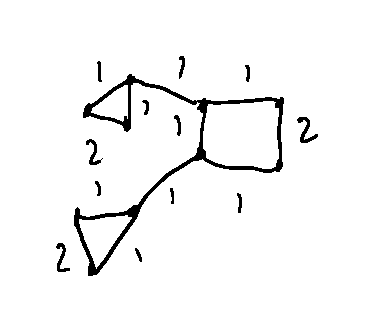
\includegraphics[width=.7\textwidth]{i1.pdf} In this case, $c=3$.
                \paragraph{Example 7}
                $G=(V,E)$ undirected graph degree of every vertex is
                $10$. Suppose to every vertex $v \in V$ a positive integer
                $a_v$ is assigned.
                \\ If $\sum_{v\in V}a_v = 5$ then what is $\sum_{u\in v}
                \sum_{\substack{w\in V:\\ uw\in E}} a_w = ? =\sum_{w \in
                  V}10a_w = 10 \times 5 =50$. Each $a_w$
                appears in the sum $10$ times since the degree of each
                vertex is $10$.
           \subsection{Topics Covered}
                The following are the topics we will be covering in
                this course:
                \begin{itemize}
                \item Network flows (More of like a practice topic for
                  what we'll be seeing in the course, will use the
                  algorithm to solve this problem for seemingly
                  unrelated problems. We'll be doing this a lot in the
                  course, called reduction, where we reduce solving
                  one problem to another problem.)
                \item Linear Programming (Bunch of constraints and
                  want to optimize a linear function). This will be
                  one of the most important concepts we learn in this
                  course.
                \item Midterm
                \item Linear Programming again
                \item NP-Completeness (no good algorithms for problems
                  that seem very basic, useful skill to have even if
                  you aren't a theoretician)
                \item Approximation algorithms (settling for the next
                  best thing for NP-Complete problems, might be able
                  to find an algorithm that approximates things, not
                  exactly optimal, but some sort of factor of how good
                  the approximation is; lots of research happening in
                  this area, better and better approximations). Will
                  use a lot of linear programming here.
                \item Randomized algorithms (randomness can actually
                  help us; probability theory/knowledge of random
                  variables may help a little bit here, but this is
                  the last stretch of the course and not very essential)
                \end{itemize}
         \subsection{Network Flows \\ Max Flow Problem}
            Very important, used in things like game theory.
            \underline{Def}: A flow is a \underline{directed} graph
            $G=(V,E)$ such that:
            \begin{enumerate}
            \item Every edge $e$ has a capacity $c_e \geq 0$.
            \item There is a source $s \in V$.
            \item There is a sink $t \in V$ such that $t\neq s$.
            \end{enumerate}
            \paragraph{Example}~\\
                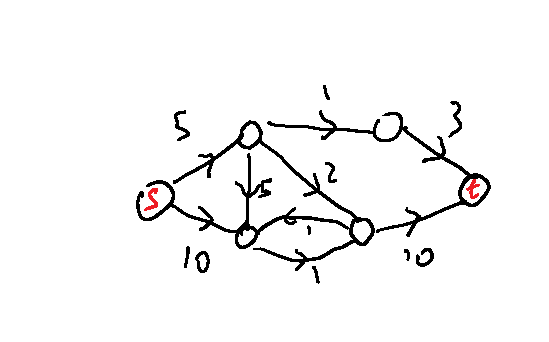
\includegraphics[width=.7\linewidth]{i2.pdf}
            \paragraph{Remark}: For the sake of convenience we make
            the following assumptions.
            \begin{enumerate}
            \item No edge enters the source.
            \item No edge leaves the sink.
            \item All capacities are integers.
            \item There is at least one edge incident to every vertex.
            \end{enumerate}
            \underline{Def}: [flow] A flow is a function $f:E
            \rightarrow \mathbb{R}^+$ such that: (Note that :$\mathbb{R}^+ = \{X \in
            \mathbb{R} | x \geq 0\}$)
            \begin{enumerate}[(i)]
            \item \text{[capacity]} $\forall e \in E, 0 \leq f(e) \leq
              c_e$ (flow cannot be negative nor can it exceed
              capacity)
            \item \text{[conservation]} For every node $u$ other than
              source and sink the amount of flow that goes into $u=$
              the amount of flow that leaves $u$. Formally:
              $$\forall u \in V\setminus\{s,t\} \underbrace{\sum_{vu\in E}f(uv)}_{f^{\text{in}}(u)} = \underbrace{\sum_{uw\in E}f(uw)}_{f^{\text{out}}(u)}$$
            \end{enumerate}
            \paragraph{Example}~\\
                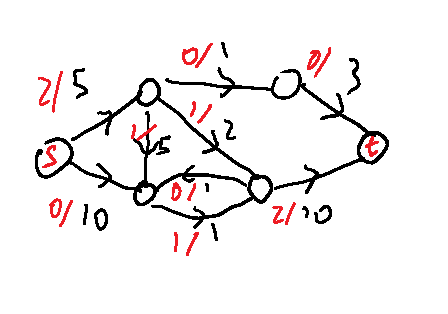
\includegraphics[width=.7\linewidth]{i3.pdf}
            \\ \underline{Def}: $Val(f) = \sum_{su\in E} f(su) =
            f^{\text{out}}s$
            \\\noindent\rule{\textwidth}{0.5pt}
            Max Flow Problem: Given a flow network find a flow with
            largest possible value.
\end{document}
